\section{Durchführung}
\label{sec:Durchführung}

\subsection{Justage der Laserdiode}
Zu Beginn soll die geringste Stromstärke gefunden werden, bei welcher ein Laserstrahl entsteht.
Die Laserdiode wird zunächst auf den optischen Tisch positioniert und eine Spannung angelegt, sodass ein Injektionsstrom fließt.
Da der Lichtstrahl mit einer Wellenlänge von $\SI{775}{\nm}$ bis $\SI{800}{\nm}$ \cite{sanyo} im Infrarotbereich liegt, wird er mithilfe einer Infrarot (IR) Detektionskarte sichtbar gemacht.
Wie in Abbildung \ref{abb:afig1} gezeigt, wird zudem eine CCD Kamera verwendet, um den Strahl auf dem angeschlossenen Bildschirm noch besser erkennen zu können.

\begin{figure}
    \centering
    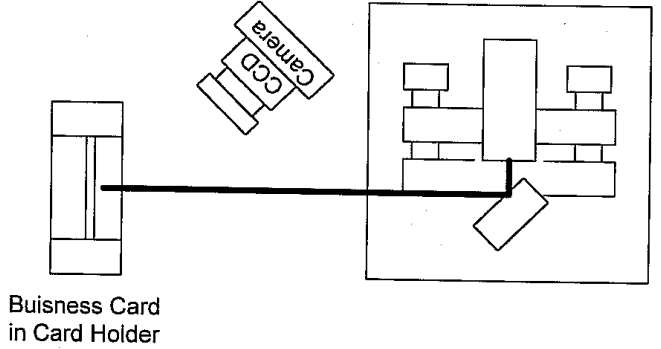
\includegraphics[width=0.7\textwidth]{pics/aufbau1}
    \caption{Versuchaufbau zur Justage des externen Resonators \cite{anleitung}. }
    \label{abb:afig1}
\end{figure}

Der Injektionsstrom wird nun so eingestellt, dass die optischen Verluste des Lasers geringer sind als die Intensitätssteigerung durch induzierte Emissionen.
Denn nur dann kann ein Laserstrahl entstehen.
Auf der IR Karte kennzeichnet sich das Lasen durch eine Auffächerung des Lichtstrahls in ein Interferenzmuster.
Dieses entsteht durch Überlagerungen des von der Karte reflektierten Lichts.
Der Injektionsstrom soll nun so eingestellt werden, dass sich der Laser genau auf der Schwellen zum Lasen befinden und weiterhin ein aufgefächerter Strahl beobachtet wird.
In Abbildung \ref{abb:afig2} ist die Auffächerung des Strahls beim Übertreten der Schwelle zum Lasen deutlich zu sehen.

\begin{figure} 
    \centering
    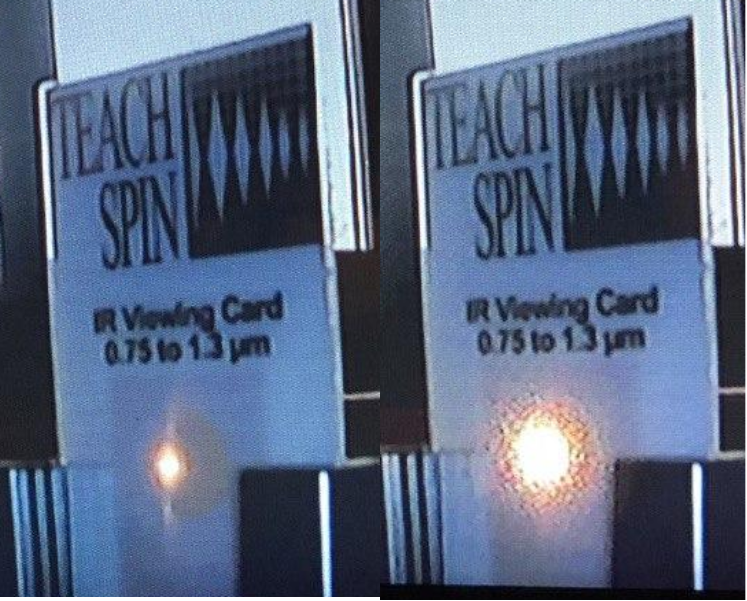
\includegraphics[width=0.5\textwidth]{pics/Lasen}
    \caption{Aufnahme des Lichtstrahls auf der IR Karte vor und nachdem der Injektionsstrom die Schwelle erreicht und der Laser zu lasen beginnt.}    
    \label{abb:afig2}
\end{figure}

Anschließend wird an dem TOP-Drehknopf der Laserdiode der Winkel des Gitters und Abstand zum Dioden-Chip eingestellt.
Dabei durchläuft die Intensität des Laserstrahls mehrere Intensitätsmaxima.
Der Drehknopf wird auf eines dieser Maxima eingestellt. 
Anschließend wird die angelegte Spannung erneut reduziert, sodass sich der Injektionsstrom wieder genau auf der Schwelle zum Lasen befindet.
Diese Prozedur wird mehrmals wiederholt, bis sichergestellt ist, dass die untere Grenze des Injektionsstroms erreicht ist.
Es wurde eine Schwellspannung von $\SI{4,43}{\V}$ erreicht, was bei einem Innenwiderstand von $\SI{100}{\ohm}$ der Stromquelle einem Injektionsstrom von $\SI{34,3}{\mA}$ entspricht.

\subsection{Aufnahme des Fluoreszenzspektrums von Rubidium}
Um das Fluoreszenzspektrums von Rubidium beobachten zu können, wird der Versuchaufbau in Abbildung \ref{abb:afig3} verwendet.
Der Laserstrahl durchläuft eine Rubidiumprobe und trifft anschließend auf die IR Karte, sodass Reflektionen im Raum vermieden werden.
Hierbei wird das Rubidiumgas konstant bei einer Temperatur von $\SI{50}{\celsius}$ gehalten.
Die CCD Kamera ist auf eine seitliche Bohrung der Apparatur gerichtet, durch welche das Fluoreszenzlicht aufgenommen wird.

\begin{figure}
    \centering
    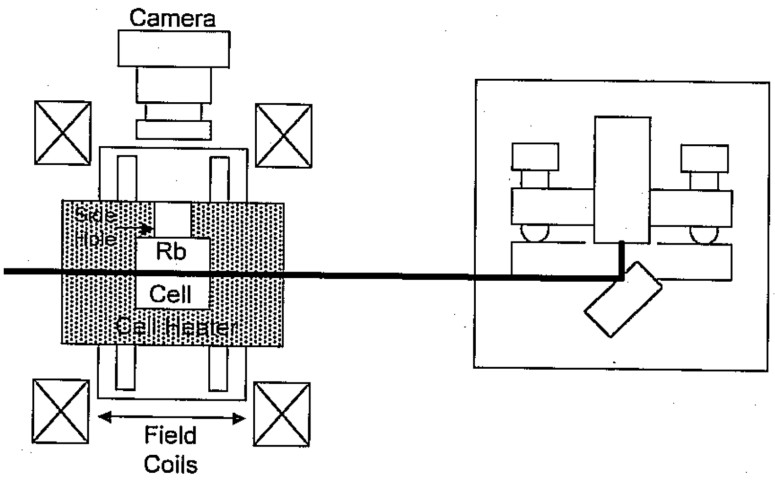
\includegraphics[width=0.7\textwidth]{pics/aufbau2}
    \caption{Versuchaufbau zur Beobachtung des Fluoreszenzspektrums von Rubidium \cite{anleitung}.}
    \label{abb:afig3}
\end{figure}

Um das Fluoreszenzlicht beobachten zu können, wird der Injektionsstrom leicht erhöht und das Gitter des externen Resonators mithilfe des SIDE-Knopfes vorsichtig horizontal verschoben.
Sobald der Laserstrahl eine Wellenlänge von $\SI{780}{\nm}$ erreicht, werden die Rubidiumatome durch Absorption eines Photons angeregt und durch die anschließende Emission der Photonen wird ein heller Lichtstreifen auf der Kamera sichtbar.
Das Fluoreszenzlicht in Form dieses Lichtstreifens ist in Abbildung \ref{abb:afig4} zu sehen.

\begin{figure}
    \centering
    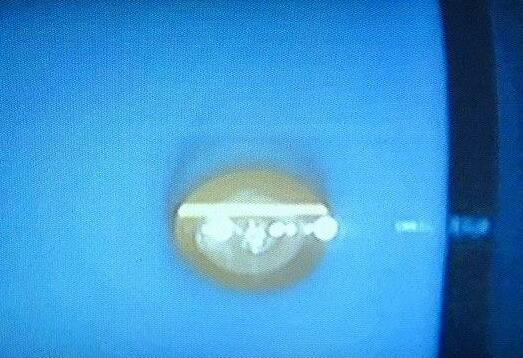
\includegraphics[width=0.5\textwidth]{pics/fluor}
    \caption{Aufnahme des Fluoreszenzlichts von Rubidium.}
    \label{abb:afig4}
\end{figure}

Um das Fluoreszenzspektrum aufzunehmen wird ein RAMP-Generator mit einer Frequenz von $\SI{10}{\Hz}$ verwendet um das Gitter des externen Resonators zu verschieben und somit die Wellenlänge des Lasers stetig zu verändern.
Dazu wird der Generator an einen Piezo Kristall angeschlossen, welcher die Position des Gitters steuert.
Das Signal des Generators wird auf einem Oszilloskop sichtbar gemacht.
Um die Intensität des Laserstrahls nach Durchqueren des Rubidiumgases zu messen, wird die IR Karte durch eine Photodiode ersetzt, dessen Signal ebenfalls auf dem Oszilloskop abgebildet wird.
Zusätzlich wird ein Neutraldichtefilter in den Strahlengang platziert um eine Übersättigung der Photodiode zu vermeiden.

\begin{figure}
    \centering
    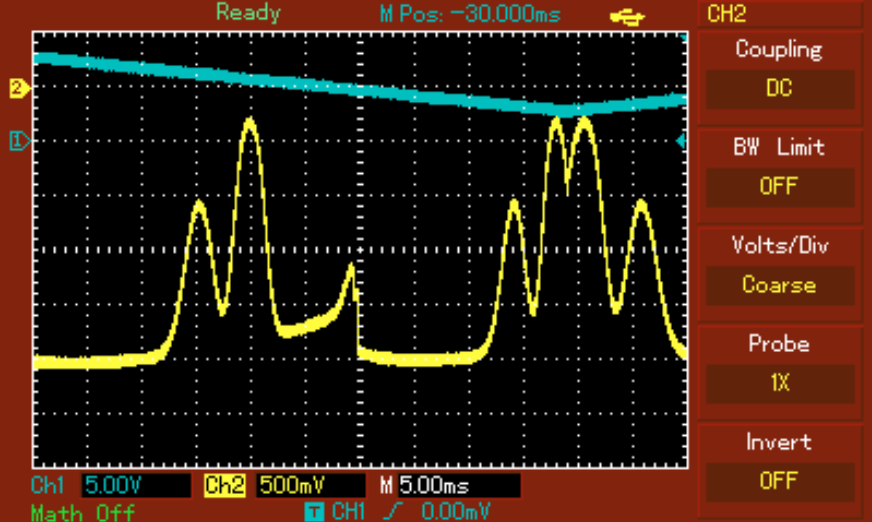
\includegraphics[width=0.6\textwidth]{data/rub1}
    \caption{Bildschirmaufnahme des Oszilloskops. Sichtbar sind die Absorptionssenkungen bei den Resonanzen des Rubidiumgases, sowie ein Modensprung in der Mitte der Aufnahme.}
    \label{abb:afig5}
\end{figure}

Abbildung \ref{abb:afig5} zeigt das erhaltene Bild des Oszilloskops.
Hierbei wurde auf die absteigende Flanke des RAMP-Generators getriggert, welcher in der Abbildung als blaue Kurve dargestellt ist.
Das grüne Signal der Photodiode zeigt die Resonanzenstellen des Rubidiumgases.
Hierbei ist zu beachten, dass diese Daten invertiert zu verstehen sind, sodass jeder Peak eine Abnahme der Intensität des Laserlichts bedeutet.
Dieser Intensitätsverlust kommt dadurch zustande, dass die Rubidiumatome Photonen absorbieren und anschließend in alle Raumrichtungen emittieren, sobald das Laserlicht einer Resonanzfrequenz entspricht.
Bei einem Durchlauf des Generators kommt es zu Modensprüngen, welche im Fluoreszenzspektrum als Zacken erkennbar sind.

\begin{figure}
    \centering
    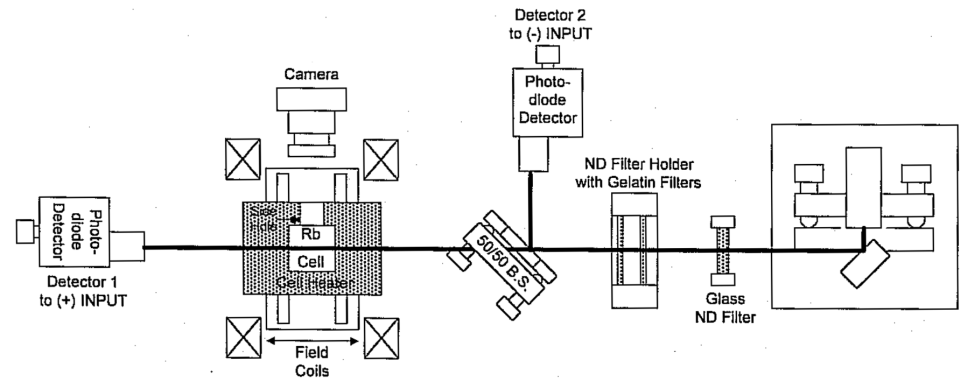
\includegraphics[width=\textwidth]{pics/aufbau3}
    \caption{Versuchaufbau zur Aufnahme des Fluoreszenzspektrum \cite{anleitung}.}
    \label{abb:afig6}
\end{figure}

Um mehr als zwei Absorptionssenkungen beobachten zu können, wird der Versuchaufbau in Abbildung \ref{abb:afig6} verwendet.
Zusätzlich zur Variation des Gitterabstandes durch den Piezo Kristall wird nun auch der Injektionsstrom mithilfe des RAMP-Generator variiert.
Das sich daraus ergebene Bild auf dem Oszilloskop ist in Abbildung \ref{abb:afig7} zu sehen.
Durch die Variation des Injektionsstroms verändert sich auch die Laserintensität stetig, sodass in der Intensität ein Grundrauschen in Form einer Dreieckspannung zu sehen ist.
Um diesen Effekt zu beheben, wird ein Strahlteiler in den Strahlengang gebracht und die Intensität des reflektierten Strahls mit einer zusätzlichen Photodiode vermessen.
Indem die Photodioden anschließend gegeneinander balanciert werden, wird die Hintergrundintensität entfernt, sodass sich auf dem Oszilloskop ein Bild ergibt, wie es in Abbildung \ref{abb:afig8} zu sehen ist.
Im Intensitätsverlauf sind die drei Intensitätssenkungen 87b, 85b und 85a aus Abbildung \ref{} deutlich zu erkennen.
Die letzte Resonanzstelle 87a zeichnet sich nur leicht ab, da diese bereits in Abbildung \ref{} eindeutig weniger stark ausgeprägt ist als die anderen.

\begin{figure}[H]
    \begin{subfigure}{0.49\textwidth}
    \centering
    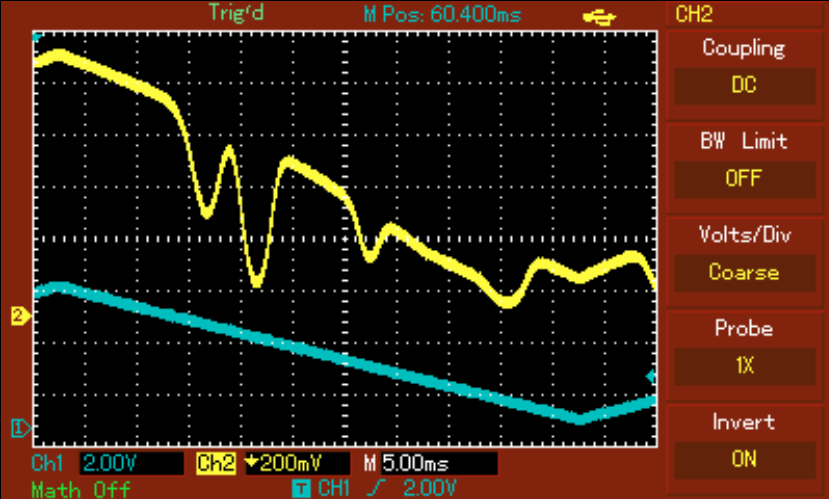
\includegraphics[width=\linewidth]{data/rub2}
    \caption{Intensitätsmessung mit Hintergrundintensität welche durch die Variations des Injektionsstroms entsteht.}
    \label{abb:afig7}
    \end{subfigure}
    \begin{subfigure}{0.49\textwidth}
    \centering
    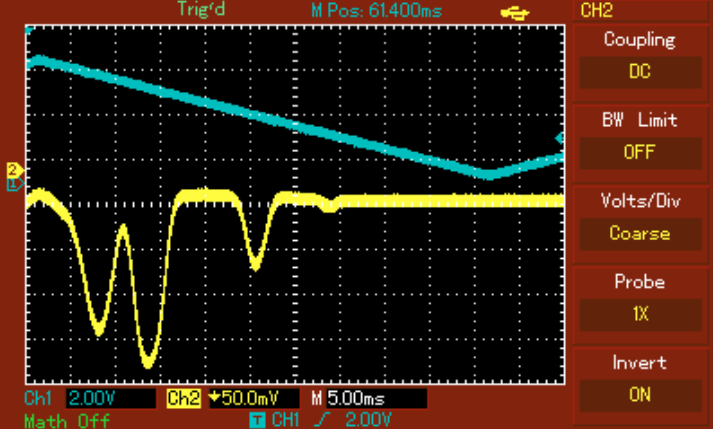
\includegraphics[width=\linewidth]{data/rub3}
    \caption{Intensitätsmessung ohne Hintergundintensität, welche mithilfe einer weiteren Photodiode entfernt wurde.}
    \label{abb:afig8}
    \end{subfigure}
    \caption{Bildschirmaufnahme des Oszilloskops. Zu sehen sind die Absorptionssenkungen des Rubidiums sowie das Sägezahnsignal des RAMP-Generators.}
\end{figure}
